\classheader{2018-06-28}
\subsection*{Autonomous Equations and Population Dynamics}
{\large \underline{Equilibrium Solutions}}\\
At any place $y_0$ where $f(y_0) = 0$, then $y'(t) = 0$ here, and thus $y(t) = y_0$ is a constant solution (or equilibrium, or steady-state solution). Its graph is a horizontal line is an isocline.\\
\redhline
\begin{equation*}
	\dfrac{dz}{dt} = z(1-z)
\end{equation*}
\begin{center}
	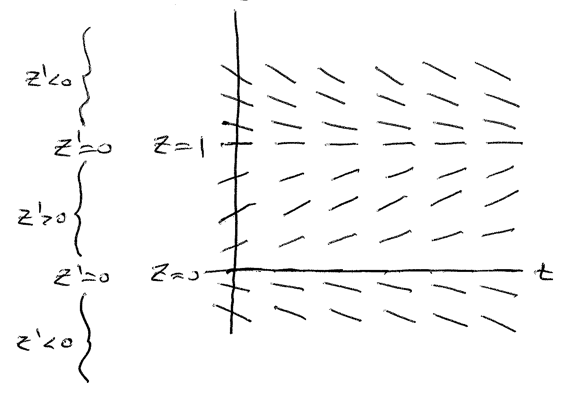
\includegraphics{7-1}
\end{center}
Here $Z(t) = 0$ and $z(t) = 1$ are both equilibrium solutions.\\
And between the equilibria, the \underline{sign} of $z'$ \underline{does not choose}. Hence solutions
\begin{enumerate}[label=\protect\circled{\Alph*}]
	\item are trapped between equilibria, and
	\item always travel in the same direction.
\end{enumerate}
In the example, we can say the following without solving:
\begin{enumerate}[label=\protect\circled{\Roman*}]
	\item Solutions exist and are unique everywhere ($f(z)$ and $f'(z)$ are polynomials)
	\item Equilibria only at $z=0$ and $z=1$.
	\item Any solution that pushes through $0 < Z_0 < 1$ will find toward the equilibria $z(t) = 1$.\\
		Any solution that starts at $Z_0 < 0$ will tend to $-\infty$\\
		Any solution that starts at $Z_0 > 1$ will tend to $z(t) = 1$\\ 
		Hence we can say
	\begin{equation*}
	\lim_{t \to \infty}z(t) = 
		\begin{cases}
			-\infty & Z_0 < 0\\
			0 & Z_0 = 0\\
			1 & Z_0 > 0
		\end{cases}
	\end{equation*}
\end{enumerate}
\redhline\\

{\large \underline{Phase Line}}\\
Any vertical slice through the slope field gives you all information about long term behavior solution:
\begin{center}
	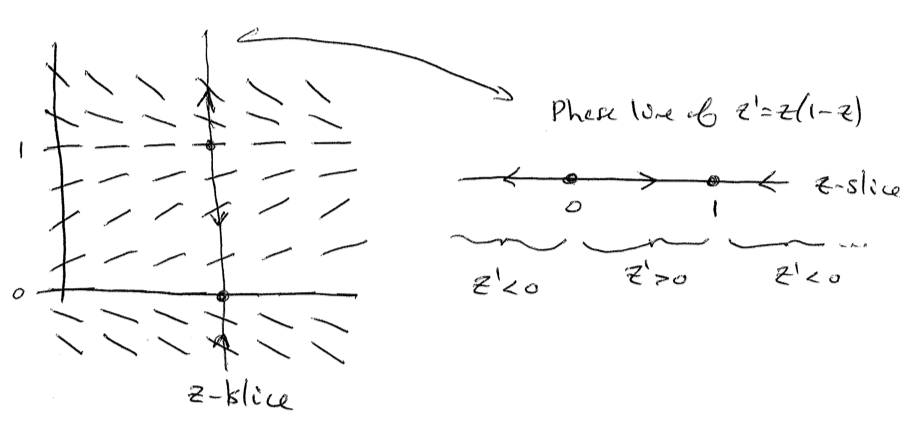
\includegraphics{7-2}
\end{center}
Here, the phase line is a schematic that determines all long term behavior of all autonomous $z'=f(z)$\\
Without a slope field still easy to see phase line: Graph $f(z)$: $z' = z(1-z) = f(z)$
\begin{center}
	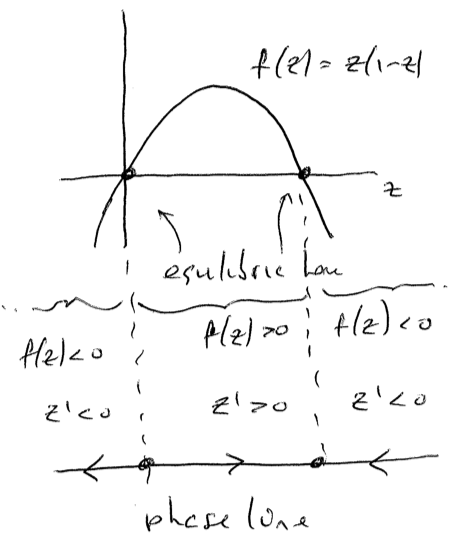
\includegraphics[scale=0.8]{7-3}
\end{center}
\begin{definition-N}
	For $y' = f(y)$, the set $\{ y \in \mathbb{R} \big| f(y) = 0\}$ is the set of \underline{critical points} for the ODE. (equilibrium solutions.)
\end{definition-N}
Critical points (equilibrium solutions) can be classified by how solutions behave around them:\\
Let $y_{\star}$ be a critical point for $y'=f(y)$ and let $N_{\varepsilon}(y_{\star}) = \{y \in  \mathbb{R} \big| |y - y_{\star} | < \varepsilon\}$ be an $\varepsilon-$neighborhood of $y_{\star}$.
\begin{enumerate}[label=\protect\circled{\alph*}]
	\item If there is a $\varepsilon > 0$ where for all $y \in N_{\varepsilon}(y_{\star})$
	\begin{equation*}
		\lim_{t \to \infty} y(t) = y_{\star} \Rightarrow \text{ is \underline{aymptotically stable}}
	\end{equation*}
	\item If there is an $\varepsilon > 0$ where for all $y \in N_{\varepsilon}(y_{\star})$
	\begin{equation*}
		\lim_{t \to -\infty} y(t) = y_{\star} \Rightarrow \text{ is \underline{unstable}}
	\end{equation*}
	\item If asymptotically stable on one side and unstable on the other, then $y_{\star}$ is semi-stable.
\end{enumerate}
\begin{example-N}
	$z' = z(1-z),$ Here critical points are $z = 0, 1$. And here $z(t) = 1$ is asymptotically stable and $z(t) = 0$ is unstable.
	\begin{center}
		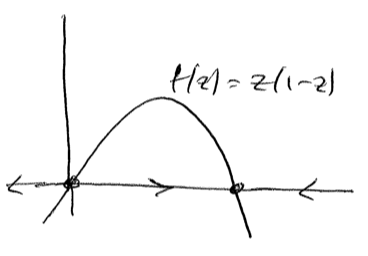
\includegraphics{7-4}
	\end{center}
\end{example-N}
\redhline\\
\begin{example-N}
	$y' = (1-y)^2 (y-4)$\\
	Here, critical points at $y=1,4$. The phase line is...
	\begin{center}
	\begin{tikzpicture}
		\draw (0,0) -- (6,0) ;
		\foreach \i in {1, 4}
			\draw (\i,0.1) circle + (0,-0.2) node[below] {$\i$};
		\foreach \i in {1, 4}
			\fill[red] (\i,0) circle (0.6 mm);
		\foreach \i in {0.5, 2.5}
			\draw (\i,0.1) circle + (0,-0.1) node[below, color=red] {$<$};
		\foreach \i in {5}
			\draw (\i,0.1) circle + (0,-0.1) node[below, color=red] {$>$};
	\end{tikzpicture}
	\\$y(t) = 4$ is unstable\\
	$y(t) = 1$ is semistable	\\
	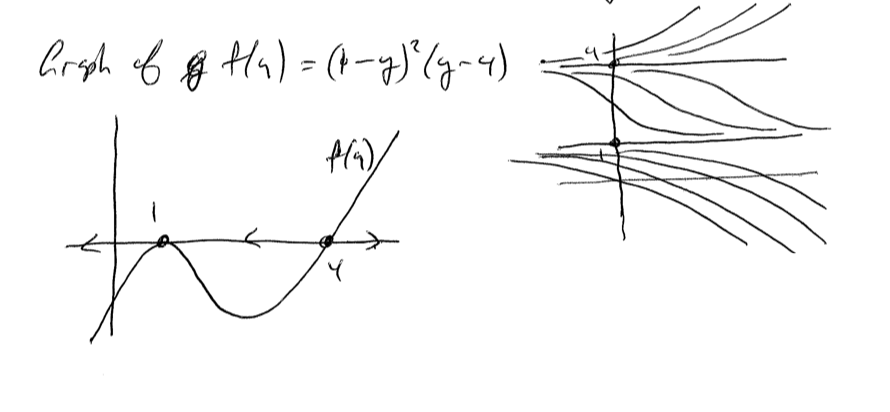
\includegraphics{7-5}
	\end{center}
	\begin{equation*}
		\lim_{t \to \infty} y(t) = 
		\begin{cases}
			\infty & y_0 > 4\\
			4 & y_0 = 4\\
			1 & 1 \leq y_0 < 4\\
			-\infty & y_0 < 1
		\end{cases}
	\end{equation*}
\end{example-N}
When graphing the $f(y)$ in $y'=f(y)$ and is constructing phrase lines, some patterns develop:\\
Let $y_{\star}$ be an equilibrium for $y'=f(y)$ (thus $f(y_{\star}) = 0$).\\
For $y$ "near" $y_0$, $y' = f(y) \cong \underbrace{ \cancelto{0}{f(y_{\star})} + f'(y_{\star}) (y-y_{\star})}_{\text{1st Taylor approx. to f(y) at } y_{\star}}$\\
{\large \textbf{Case 1:}} Suppose $f'(y_{\star}) > 0$
\begin{center}
	$\Rightarrow$ for $y>y_{\star}, \quad y'>0$
and $y < y_{\star}, \quad y' < 0$
\end{center}
\begin{center}
	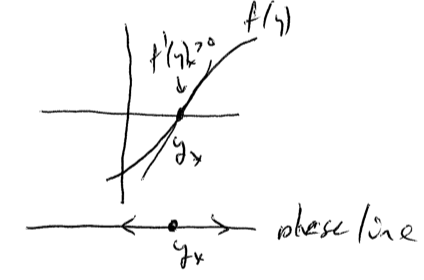
\includegraphics{7-6}
\end{center}
All nearby solutions move away $\Rightarrow y_{\star}$ is on unstable node or source\\
{\large \textbf{Case 2:}} Suppose for $f'(y_{\star}) < 0$
\begin{equation*}
	\Rightarrow \text{ for } y>y_{\star}, \quad y'<0 \text{ and } y < y_{\star}, \quad y' > 0
\end{equation*}
\begin{center}
	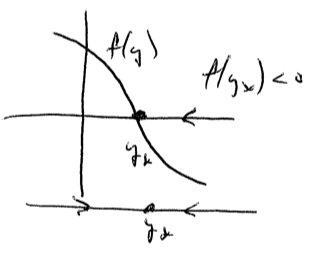
\includegraphics{7-7}
\end{center}
All nearby solutions converge to $y_{\star} \Rightarrow$ asymptotically stable on \underline{sink.}\\
{\large \textbf{Case 3:}} $f(y_{\star}) = 0$. Need more information.